\section{Un Réseau}

\paragraph{Réseaux naturels, n\oe{}uds, liens}

\paragraph{} Bien que le terme de réseau ne se soit largement démocratisé que depuis quelques dizaines d'années, il tire ses
racines plus anciennes du latin \emph{resel} qui signifiait \emph{le filet}. On retrouve ici la caractéristique
principale du réseau : ce sont des \emph{n\oe{}uds liés} entre eux selon un \emph{schéma}. Les réseaux existent en
premier lieu sous forme naturelle, on pense alors aux cours d'eau et à leurs conjonctions, aux mouvements de troupeaux,
aux racines des arbres. Nous remarquons que les constructions humaines suivent également des réseaux : le réseau routier
avec les villes comme n\oe{}uds, le réseau ferré et les gares, le réseau électrique et les centrales...

\paragraph{} Toute création regroupant des n\oe{}uds avec des relations entre ces n\oe{}uds peut être qualifiée de "Réseau". En sciences,
la discipline qui s'occupe d'étudier les réseaux, et qui regroupe mathématique et informatique, s'appelle
la \emph{Théorie des Graphes}. Lorsque toute relation entre deux n\oe{}uds d'un graphe est symétrique, c'est à dire qu'elle va
dans un sens et dans l'autre, nous parlons de graphes \emph{non orientés}. Ce n'est par exemple pas le cas pour le
réseau routier qui est un graphe \emph{orienté}, car il possède des rues \emph{à sens unique}.

\begin{figure}[h]
    \centering
    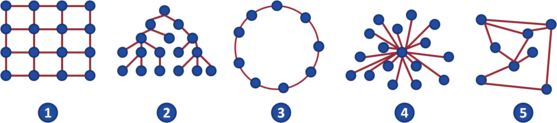
\includegraphics[width=400px]{chapters/02/images/reseaux.png}
    \caption{\label{Réseaux, graphes} Différentes formes de graphes}
\end{figure}

\paragraph{} On peut retrouver naturellement certaines de ces constructions. Le réseau hiérarchique (2) existe
au sein des sociétés, des gouvernements et des groupes d'Hommes en général. Il décrit généralement une structure
de contrôle par le haut, où le n\oe{}ud le plus haut est dit \emph{parent} des n\oe{}uds juste en dessous, et ainsi de suite.
Ainsi le pouvoir se concentre sur le haut du réseau et peut facilement être transmis verticalement, mais pas de 
manière transverse.

\paragraph{} On retrouve également le réseau centralisé (4) dans les organisations humaines par exemple,
où il traduit simplement la référence directe à un pouvoir supérieur. Les n\oe{}uds n'ont pas besoin de connaître
l'existence d'autres n\oe{}uds car ils se réfèrent directement à une unité centrale qui sera \emph{décisionnaire}.
Souvent, les réseaux centralisés forment entre eux d'autres réseaux centralisés plus importants afin de reléguer
toute les \emph{micro-décisions} à une entité centrale supérieure qui sera en charge, à partir de ces informations,
de calculer une \emph{macro-décision}. On retrouve ici la notion de \emph{couches}, qui nous servira dans l'étude
de réseaux plus complexes.

\paragraph{} Par opposition à la centralisation, le réseau décentralisé (5) est à l'image d'un système décisionnaire au
sein duquel chaque participant peut faire entendre sa voix. Il n'est pas nécessaire pour un participant d'avoir connaissance
de l'ensemble des membres du réseau, car l'information est transmise de n\oe{}ud en n\oe{}ud, à travers le maillage.
Cela permet notamment de mettre en place des réseaux beaucoup plus résilients : si l'un des n\oe{}uds est déconnecté,
le réseau peut continuer de fonctionner.


\paragraph{Types de réseaux}

\paragraph{} En informatique, lorsque plusieurs machines sont connectées entre elles, le plus souvent par des câbles, on
parle alors de \emph{réseau}. Afin de comprendre pourquoi certaines topologies de réseaux existent, nous allons introduire 
deux types de réseaux bien connus : \emph{le LAN et le WAN}.

\paragraph{} Le LAN, ou Local Area Network, se limite à un espace géographique déterminé. On peut prendre
par exemple le contenu d'une salle, un étage, un immeuble. Ainsi les réseaux d'une école, d'un
hopital, d'une gare, d'un aéroport, sont des LANs. Pour parler de transmission sans fil, ou
Wi-Fi, on utilise aussi le terme \emph{WLAN}, pour Wireless LAN. Les points d'accès Wi-Fi, qui se
sont démultipliés dans les cafés, restaurants, lieux d'attente, aéroports à travers le monde
sont des exemples de WLAN.

\paragraph{} Le WAN signifie Wide Area Network, ou réseau étendu. Il est en fait formé par
l'association de plusieurs LANs. On retrouve ici la notion de réseaux \emph{composés}. Des LANs,
reliés entre eux, forment un réseau à part entière, qui peut lui même se connecter à d'autres
LANs ou WANs.


\paragraph{Réseau nominal} 

\paragraph{} Aujourd'hui, les réseaux informatiques que nous utilisons au quotidien sont composés
de l'exacte manière que nous venons de présenter : une multitude de - plus ou moins - petits LANs, et un empilement
par couches successives de WANs dont le dernier, \emph{internet}, les met tous en relation. Il est inutile de divaguer
sur la mise en place d'un \emph{réseau universel}, car celui-ci est déjà en place. Omniprésent, nous l'utilisons au
quotidien.

\paragraph{} Il serait normalement nécessaire de prendre en considération les aspects liés à la gouvernance de ce réseau 
mondial, entre intérêts des États et des opérateurs de télécommunication. Mais nécessaire uniquement s'il était question
de \emph{prendre contrôle} du réseau ; hors ce n'est pas de cela qu'il s'agit. Car contrôler le réseau implique des 
responsabilités, tandis qu'en tirer parti n'entraîne - virtuellement - que des avantages.

\paragraph{} Mais quand on parle de réseau, il est important de ne pas s'arrêter qu'au sens \emph{physique}, matériel du
terme. Car sur un même réseau physique peuvent cohabiter une multitude de réseaux logiques - \emph{logiciels}. C'est cet
aspect des réseaux qui va nous intéresser plus particulièrement, car si un réseau physique est un \emph{moyen}, un réseau
logique a une \emph{fin}.

\paragraph{} Sur ce réseau nominal vont être mis en place une multitude de réseaux logiques fournissant des services à
leurs utilisateurs. Cependant, la nature \emph{centralisée} de ces réseaux rend aisé la mise en place d'une censure de
l'information, quelle qu'elle soit. De même, l'utilisateur n'a d'autre choix que de faire \emph{confiance} à l'entité
lui fournissant un service en ce qui concerne les données qu'elle transmet.

\paragraph{} Et bien souvent, entre l'utilisateur et le service, on retrouve un acteur incontournable : le moteur de
recherche. Le rôle de ce service est double : il va dans un premier temps \emph{indexer} le plus de contenus possible
accessible sur internet, et dans un second temps permettre à un utilisateur d'effectuer une recherche par mots clés 
pour lui renvoyer les contenus jugés les plus appropriés. Certains moteurs, plus spécifiques, utilisent leur base
d'indexation pour fournir non plus un \emph{contenu} brut mais un ensemble de \emph{connaissances} liées à la requête
de l'utilisateur \cite{Internet2}.

\paragraph{} Le rôle à jouer des moteurs de recherche dans l'écosystème technologique actuel est colossal : ils peuvent
presque être considérés comme la "porte" d'internet, permettant de trouver un contenu approprié à notre besoin en quelques
instants. Mais encore une fois ce service est à double tranchant, car les résultats renvoyés par le moteur sont fonction
du contenu de sa base d'indexation. De fait Tim Bray, ancien employé de Google travaillant aujourd'hui chez Amazon Web Services,
a remarqué que certains vieux articles de blogs étaient devenus, début 2018, totalement introuvables en utilisant le plus
important moteur de recherche mondial... alors que les résultats ressortaient bien sur d'autres services et que les pages 
étaient évidemment toujours accessibles \cite{Internet3}.

\paragraph{} Il ne s'agit là que d'un exemple, mais il met en exergue le déséquilibre de la balance des pouvoirs dans un 
modèle centralisé, dans lequel les n\oe{}ud périphériques (les utilisateurs) sont dépendant du n\oe{}ud central (fournissant
le service).


\paragraph{Réseaux parallèles}

\paragraph{} C'est ce constat qui a servi de base au développement de réseaux dits \emph{parallèles}. Il nous est
impossible d'en donner une définition exacte ; en effet, chacun va adresser une solution à un problème particulier,
offrant une alternative voire induisant une évolution des usages dans le domaine concerné.

\paragraph{} Cependant, il est important de bien faire dès à présent la distinction entre un \emph{réseau parallèle} et 
ce que l'on se complait à appeler le "\emph{deep web}". En effet, le terme "réseau profond" ne
désigne rien de plus que le contenu non indexé par les moteurs de recherche sur internet. Il ne s'agit en aucun cas d'un
réseau alternatif nécessitant une manipulation technique particulière pour y accéder : il vous suffit de saisir le nom de
domaine ou l'adresse IP en question dans la barre d'adresse de votre navigateur pour y accéder.

\paragraph{} La notion de \emph{dark web} fait quant à elle son apparition dans le langage journalistique courant avec la 
démocratisation du réseau Tor (\emph{The Onion Router} \cite{Internet4}), permettant d'anonymiser un canal d'échange en chiffrant
le flux et en le faisant transiter par un ensemble non déterminé de relais avant d'arriver à destination. Cette technologie
offre plusieurs avantages : 

\begin{itemize}
    \item C'est un moyen de contourner la censure : si un opérateur ou un État prend la décision de couper ou restreindre
    l'accès à un service, celui-ci sera toujours accessible à traver le réseau Tor ;
    \item Il permet de protéger les utilisateurs des attaques \emph{Man in the Middle} (MitM), consistant pour l'attaquant
    à venir se placer entre le flux de la victime et le serveur de destination pour y récupérer des informations ;
    \item Le trafic passant à travers un ensemble de relais avant d'arriver à destination, les seuls informations personnelles
    qui pourront vous être subtilisées seront celles que \emph{vous} donnez ;
    \item Il est possible de rendre un service (site web) accessible uniquement à travers le réseau Tor en utilisant une
    adresse en \lstinline{.onion}.
\end{itemize}

\paragraph{} Cette dernière fonctionnalité, désormais baptisée \emph{onion services} - en référence au système de routage
multi-couches du projet -, était auparavant appelée \emph{hidden services} \cite{Internet5}. Ce sont ces services "cachés",
car accessibles uniquement à travers le réseau Tor, qui firent émerger la notion de réseau parallèle "sombre" car non 
accessible par des moyens conventionels.

\paragraph{} Bien que l'utilisation d'un tel réseau parallèle et de ses services cachés aille bien souvent de paire dans 
l'imaginaire collectif avec des activités illégales - dont la plus retentissante affaire concerna \emph{Silk Road}, un 
site commercial permettant l'achat et la vente de services illégaux entre utilisateurs - ce rapprochement, s'il est tranché, est inutilement
simpliste. Ainsi, le réseau social Facebook, le Service National de Police et des Poursuites Publics du Pays-Bas \cite{Internet6}
ou encore le New York Times \cite{Internet7} ont chacun lancé leur propre \emph{onion service}, en facilitant l'usage par 
les utilisateurs du réseau Tor.

\paragraph{} Car au delà des services "exclusifs" présents sur le réseau, c'est surtout sa fonctionnalité d'anonymisation
des flux qui le rend indispensable pour certaines utilisations. Nous citerons l'exemple bien connu des lanceurs d'alertes
quels qu'ils soient, qui ont ainsi la possibilité de transmettre en toute sécurité informations et documents aux médias
intéressés. Un usage moins connu est celui des forces armées, plus précisément la U.S. Navy, qui utilisa Tor pour communiquer
de manière sécurisée depuis le terrain lors de leur intervention au Moyen Orient.

\paragraph{} Mais bien évidemment, les usages illégaux de cette technologie existent eux aussi. Comment peut-on alors 
prévenir de telles dérives ? Cependant... est-ce seulement souhaitable ? En effet, la raison même de ce réseau est de
permettre à ses utilisateurs d'échapper à tout contrôle, à toute censure. Dès lors, vouloir empêcher toute dérive (encore
faudrait-il définir ce que regroupe cette dénomination !) revient à imposer un contrôle de l'utilisation faite du réseau.
Il serait alors dénaturé, et perdrait immédiatement toute attractivité, tout intérêt.

\paragraph{} Un autre acteur fait beaucoup parler de lui depuis une poignée d'années : il s'agit de la technologie 
"\emph{blockchain}", avec le Bitcoin comme fer de lance médiatique. Il convient tout d'abord de la définir, car derrière 
le terme de \emph{blockchain} se cache en réalité une certaine complexité technique, que l'on peut regrouper en quatre parties :

\begin{itemize}
    \item Un réseau décentralisé en pair-à-pair, permettant à chaque n\oe{}ud d'interagir indépendamment avec l'ensemble 
    du réseau ;
    \item Une base de données distribuée : il s'agit réellement de la \emph{blockchain}, une suite d'informations certifiées
    puis enregistrées dans des "blocs" de données chaînés les uns à la suite des autres ;
    \item Un consensus décentralisé, base commune à chaque participant du réseau servant à valider l'ensemble des informations
    qui y transitent ;
    \item Du chiffrement asymétrique, permettant à chacun de certifier les informations enregistrées dans la blockchain et
    d'en vérifier la provenance.
\end{itemize}

\paragraph{} Un fois assemblées, elles permettent de former un protocole complet (\emph{bitcoin://}). Dans le cas de Bitcoin,
ainsi que pour la grande majorité des \emph{cryptocurrencies} (cryptomonnaies, ou "monnaies cryptographiques"), le domaine d'application
de cette technologie révolutionnaire est la finance. Là où Tor fait évoluer nos échanges et interactions sur le réseau, 
les blockchains souhaitent dans un premier temps boulverser notre rapport - plus qu'à l'argent - mais à la \emph{valeur}, 
en créant une multitude de réseaux financiers parallèles ayant pour objectif de rendre obsolète l'usage du tiers de confiance
que représentent aujourd'hui les banques et autres institutions financières dans toutes les transactions à l'échelle mondiale.

\paragraph{} Il s'agit d'un réseau \emph{distribué} plus que décentralisé, ce qui signifie qu'en plus de sa décentralisation
constitutive, les données contenues dans la blockchain sont présentes sur chaque n\oe{}ud du réseau. Ainsi, ce dernier est
en capacité de se reconstituer à partir d'un unique n\oe{}ud. De même, la validation des données étant effectuée individuellement
par chaque n\oe{}ud, décidant ou non d'enregistrer les nouvelles informations sur sa base locale - mais toujours en suivant 
les règles d'un \emph{consensus commun} -, il est impossible pour un attaquant isolé de faire enregistrer des informations 
falsifiées ou de modifier le contenu de la blockchain. Car même s'il effectuait ces manipulations frauduleuses sur sa base
locale, toutes ses tentatives de réplication seraient rejettées par l'ensemble du réseau. Il existe bien entendu des vecteurs
d'attaque potentiel (attaque dite "des 51\%"), mais ceux-ci nécessitent de prendre contrôle de plus de la moitié de la puissance
de calcul du réseau, ce qui est à ce jour difficilement envisageable.

\paragraph{} Les cryptomonnaies ont longtemps été associées à un usage frauduleux : transactions illégales, blanchiment d'argent, etc.
Il est important de comprendre que si ces pratiques ont bien eu lieu, elles démontrent une profonde incompréhension de 
l'objectif comme du fonctionnement de cette technologie tout en mettant - aussi ironique que cela puisse paraitre - en 
périle les opérations illégales en question. Car l'anonymat n'existe pas dans ce monde-ci.

\paragraph{} Il conviendrait plutôt d'employer le terme \emph{pseudonymat}, ou pseudo-anonymat. Chaque utilisateur a la
possibilité de générer une quantité théoriquement infinie d'\emph{adresses}, chacune représentant schématiquement un compte
en banque. Il est alors en capacité d'effectuer des transactions, une fois qu'il aura obtenu un peu de \emph{token}, c'est-
à-dire d'unités de la cryptomonnaie en question. Cela nous fait justement approcher d'un point crucial de ce modèle : 
comment peut-on échanger de l'argent réel en échange de cryptomonnaie et inversement ? En en achetant ou en vendant à quelqu'un,
que ce soit un ami, un commerçant, ou un \emph{exchange}, ces sites spécialisés dans le trading de cryptomonnaies. Dans 
une activité illicite, la question de l'entrée et de la sortie de fonds est primordiale, or il est ici nécessaire de faire 
confiance à un autre détenteur de tokens. De plus, chaque membre du réseau possède une copie complète de l'ensemble des 
transactions effectuées : il est donc extrêmement aisé de suivre les mouvements de fonds à travers le réseau.

\paragraph{} En effet, l'objectif de cette technologie est d'abolir les privilèges inhérents à une structure centralisée :
tous les participants sont mis sur un pied d'égalité, et aucun ne possède de \emph{poids} particulier par rapport à d'autres
au sein du réseau.

\paragraph{} En mars 2016, la première version du projet Ethereum est déployée sous le nom de \emph{Homestead}. Première 
implémentation du \emph{whitepaper} dévoilé en décembre 2013 par Vitalik Buterin, son concept est révolutionnaire : permettre
de déployer dans une blockchain - en profitant ainsi de l'ensemble de ses caractéristiques techniques, de la distribution à
l'immutabilité des données - une application précompilée. Ce sont les \emph{Smart Contracts} ("contrats intelligents"),
aussi appelés \emph{Decentralized Applications}, ou \emph{ÐApps}. Voici quelques-unes de leurs propriétés intéressantes :

\begin{itemize}
    \item Une ÐApp ne nécessite aucune infrastructure pour être exécutée : une fois déployée dans la blockchain Ethereum,
    elle est accessible (et donc exécutable) depuis n'importe quel n\oe{}ud du réseau ;
    \item \emph{Lire} une information contenue dans une ÐApp est gratuit ;
    \item Modifier l'\emph{état} d'une ÐApp (enregistrer ou modifier une structure de données par exemple) représente un
    coût calculé en fonction de la complexité de l'opération effectuée ; cela permet d'assurer qu'un algorithme ne puisse
    pas boucler infiniment et que sa complexité soit optimisée de manière à en réduire le coût d'usage.
\end{itemize}

\paragraph{} En utilisant cette technologie en backend et en la couplant avec une interface mobile ou une application légère
s'exécutant côté client, il est désormais envisageable de développer des applications complètes ne nécessitant presque aucune
infrastructure : on peut imaginer que le front-end soit développé en JavaScript et déployé sur une plateforme type GitHub
Pages.

\paragraph{} Dès lors, cela offre un pouvoir de création immense pour les développeurs ou jeunes entreprises ne disposant 
pas forcément des moyens nécessaires pour louer les services d'un fournisseur de cloud publique ou pour acheter et installer
eux-même l'ensemble du matériel tout en devant en assurer l'entretien. Technologiquement comme humainement, les technologies
blockchain cassent les rapports de force instaurés par une sur-centralisation de l'ensemble des services que nous utilisons
au quotidien.

\paragraph{} Mais quel est l'avenir pour l'ensemble de ces réseaux parallèles ? Sont-il voués à disparaître, ou au contraire
à supplanter le réseau nominal pour devenir \emph{de facto} le nouveau standard ? À nôtre sens, il est illusoire de soutenir
l'une ou l'autre de ces théories, par trop manichéennes. Loins de prétendre prédire l'avenir, nous espérons assister à un 
équilibrage des rapports de force, amenant les réseaux à coexister et les services, peu à peu, à se libérer du carcan de la
centralisation pour le bien de leurs utilisateurs. Petit à petit, peut être assisterons-nous à une neutralisation du Réseau
par le Réseau, induisant à la fois une plus grande transparence de tous et une plus grande anonymité des utilisateurs.


\paragraph{Réseau... universel ?}

\paragraph{} Ainsi, puisque notre vecteur d'échange est déjà en place, 

\paragraph{TODO} "Idéal" de la mise en place d'un Réseau universel, omniprésent
et omniscient. Un tel système global impliquerait la mise en place d'un système hautement
distribué, voire \emph{"participatif"}.

\paragraph{TODO} Qu'est-ce qu'un réseau 'universel' ? Quels sont ses avantages ? Ses inconvénients ?
Qu'implique techniquement sa mise en place ? Est-ce réalisable aujourd'hui ? Qu'est-ce qu'un réseau distribué ? 